% IEEE Journal Template - 完整中文版
% 請在 Overleaf 使用 XeLaTeX 編譯 (Menu -> Compiler -> XeLaTeX)
\documentclass[journal]{IEEEtran}

% ===== XeLaTeX 中文支援 =====
\usepackage{fontspec}
\usepackage{xeCJK}

% ---- 字型：先用最穩的 Times-like + CJK 後備 ----
\setmainfont{TeX Gyre Termes} % Times-like, TeXLive/Overleaf 幾乎必有

% 字體自動切換邏輯 (Fallback)
\IfFontExistsTF{Source Han Serif TC}{
  \setCJKmainfont[AutoFakeBold=true]{Source Han Serif TC}
}{
  \IfFontExistsTF{Noto Serif CJK TC}{
    \setCJKmainfont[AutoFakeBold=true]{Noto Serif CJK TC}
  }{
    \setCJKmainfont[AutoFakeBold=true]{AR PL UMing TW}
  }
}

\IfFontExistsTF{Source Han Sans TC}{
  \setCJKsansfont[AutoFakeBold=true]{Source Han Sans TC}
}{
  \IfFontExistsTF{Noto Sans CJK TC}{
    \setCJKsansfont[AutoFakeBold=true]{Noto Sans CJK TC}
  }{
    \setCJKsansfont[AutoFakeBold=true]{AR PL UMing TW}
  }
}

% ---- 中文自動斷行（很重要）----
\XeTeXlinebreaklocale "zh"
\XeTeXlinebreakskip = 0pt plus 1pt

% 中英文間距（保守設定）
\xeCJKsetup{CJKmath=false}

% ===== 套件 =====
\usepackage{graphicx}
\usepackage{amsmath,amssymb}
\usepackage{booktabs,multirow,array}
\usepackage{xcolor}
\usepackage{listings}
\usepackage{cite}
\usepackage[hidelinks]{hyperref}

% TikZ/pgfplots（建議偏黑白/灰階）
\usepackage{tikz}
\usetikzlibrary{shapes,arrows,positioning,fit,calc,automata}
\usepackage{pgfplots}
\pgfplotsset{compat=1.17}
\usepackage{balance}
% ===== 排版舒適度優化 (修正：移除 linespread 避免 listings 錯亂) =====
% \raggedbottom % 若需要可開啟，但 IEEEtran 預設 flushbottom 較專業
% 這裡不使用 linespread，避免 vertical spacing 計算錯誤

% ===== 程式碼樣式 =====
\definecolor{codegreen}{rgb}{0,0.5,0}
\definecolor{codegray}{rgb}{0.5,0.5,0.5}
\lstdefinestyle{verilog}{
    language=Verilog,
    basicstyle=\ttfamily\tiny, % 縮小字體以適應雙欄
    keywordstyle=\color{black}\bfseries,
    commentstyle=\color{codegreen},
    stringstyle=\color{black},
    numbers=left,
    numberstyle=\tiny\color{codegray},
    numbersep=4pt,
    frame=lines,
    rulecolor=\color{black!50},
    breaklines=true,            % 自動換行
    breakatwhitespace=false,    % 允許在任何字符處換行 (重要)
    tabsize=2,
    showstringspaces=false,
    columns=fixed,              % 改回 fixed 以確保對齊正確，避免 fullflexible 導致的寬度誤判
    aboveskip=0.5em,            % 減少間距
    belowskip=0.5em,
    xleftmargin=1em             % 避免行號突出
}
\lstset{style=verilog}
% =========================
% Typography / Spacing (Final)
% =========================
\raggedbottom

% 保留 IEEE 風格但讓中文更順（不要像講義那麼鬆）
% \linespread{1.05}
\setlength{\parskip}{0.20em}

% Lists：不要 nosep（太緊）也不要太鬆；讓標題相對更醒目
\usepackage{enumitem}
\setlist{
  leftmargin=*,
  topsep=0.25em,
  itemsep=0.15em,
  parsep=0em
}

% =========================
% CJK font bold handling (reduce "fake bold looks like red-mark")
% =========================
% 只在真的沒有 Bold 字重的後備字型才用 AutoFakeBold
\IfFontExistsTF{Source Han Serif TC}{
  \setCJKmainfont[
    BoldFont={Source Han Serif TC Bold}
  ]{Source Han Serif TC}
}{
  \IfFontExistsTF{Noto Serif CJK TC}{
    \setCJKmainfont[
      BoldFont={Noto Serif CJK TC Bold}
    ]{Noto Serif CJK TC}
  }{
    \setCJKmainfont[AutoFakeBold=true]{AR PL UMing TW}
  }
}

\IfFontExistsTF{Source Han Sans TC}{
  \setCJKsansfont[
    BoldFont={Source Han Sans TC Bold}
  ]{Source Han Sans TC}
}{
  \IfFontExistsTF{Noto Sans CJK TC}{
    \setCJKsansfont[
      BoldFont={Noto Sans CJK TC Bold}
    ]{Noto Sans CJK TC}
  }{
    \setCJKsansfont[AutoFakeBold=true]{AR PL UMing TW}
  }
}

% =========================
% Consistent tags (avoid heavy bold in body text)
% =========================
\newcommand{\tagit}[1]{\textit{#1}}
\newcommand{\Goal}{\tagit{目標：}}
\newcommand{\Note}{\tagit{注意：}}
\newcommand{\Insight}{\tagit{關鍵洞察：}}
\newcommand{\ResultTag}{\tagit{結果：}}
\newcommand{\PASS}{\textsc{Pass}}
\newcommand{\FAIL}{\textsc{Fail}} % 以備不時之需（不會搶焦）

% =========================
% Tables
% =========================
\renewcommand{\arraystretch}{1.20}

% =========================
% TikZ grayscale style (Final)
% =========================
\tikzstyle{stage} = [rectangle, draw, fill=black!6, text centered, minimum height=1.5em, minimum width=2em, font=\scriptsize]
\tikzstyle{reg}   = [rectangle, draw, fill=black!3, text centered, minimum height=1em, font=\tiny]
\tikzstyle{state} = [circle, draw, fill=black!4, minimum size=1.5em, font=\scriptsize]
\tikzstyle{arrow} = [thick,->,>=stealth]

\begin{document}

\title{Pipeline MIPS 處理器之效能優化研究：\\涵蓋 13 項貢獻之綜合分析}

\author{JUNYI LIU
\thanks{Computer Architecture, National Sun Yat-sen University, December 2025.}}

\markboth{Computer Architecture Final Project Report, NSYSU, Dec.~2025}%
{Liu: Performance Optimization of a Pipelined MIPS Processor}

\maketitle

\begin{abstract}
本論文針對 5-stage pipeline MIPS 處理器進行全面性效能優化研究。我們實作並評估 13 項貢獻，包含 Data Forwarding、Branch Prediction、SIMD 平行處理、CORDIC 三角函數運算、Polynomial exp 逼近、L1~Cache，以及用於微積分運算的 ODE Solver。評估採用兩種方法：(1) \textbf{cycle-accurate RTL simulation}，使用 MiBench bitcount benchmark；(2) \textbf{analytical model-based projection}，使用 SPEC CPU2006 instruction mix ratios。結果顯示，在 MiBench 上實測達到 2.61$\times$ 加速，而在 memory-intensive SPEC workloads 上預估可達 34.84$\times$ 加速。Design of Experiments (DOE) 分析揭示 Cache 提供最大的單項改進 (2.15$\times$)，且 Cache+SIMD 展現\textbf{正向交互作用} (synergy factor 1.20 under our cost model)。
\end{abstract}

\begin{IEEEkeywords}
MIPS, Pipeline, Forwarding, Branch Prediction, Cache, SIMD, CORDIC, ODE Solver, MiBench
\end{IEEEkeywords}

%=============================================================================
\section{緒論}
現代處理器設計仰賴多種優化技術來彌補 CPU 與記憶體之間的效能差距——即所謂的「Memory~Wall」問題~\cite{hennessy2017computer}。本專案為 5-stage MIPS pipeline 實作 13 項優化。本節為不熟悉計算機架構概念的讀者提供基礎背景知識。

\subsection{什麼是 MIPS？}
MIPS (Microprocessor without Interlocked Pipeline Stages) 是一種 32-bit RISC (Reduced Instruction Set Computer) 架構，由 John Hennessy 於 1981 年在 Stanford University 開發~\cite{patterson2020computer}。MIPS 在計算機架構教育中被廣泛使用，原因如下：
\begin{itemize}
    \item \textbf{簡潔設計}：固定 32-bit 指令格式，僅有三種指令類型 (R, I, J)
    \item \textbf{教育標準}：被 Patterson \& Hennessy 教科書採用，為計算機架構之「聖經」
    \item \textbf{實務應用}：廣泛應用於嵌入式系統、路由器 (Cisco)、遊戲主機 (PlayStation 1/2) 及 IoT 裝置
\end{itemize}

\textit{MIPS 基本指令類型}：
\begin{itemize}
    \item \textbf{R-type} (Register)：\texttt{add \$t0, \$t1, \$t2} --- 暫存器之間的算術運算
    \item \textbf{I-type} (Immediate)：\texttt{lw \$t0, 0(\$t1)} --- 記憶體存取及立即值
    \item \textbf{J-type} (Jump)：\texttt{j label} --- 無條件跳躍
\end{itemize}

\subsection{5-Stage Pipeline 架構}
Pipelining 是一種允許多條指令重疊執行的技術，類似於工廠的組裝線。不同於完成一條指令後才開始下一條，每個 stage 同時處理不同的指令。

\textbf{五個 Stage 說明}：
\begin{enumerate}
    \item \textbf{IF (Instruction Fetch)}：使用 Program Counter (PC) 從記憶體讀取指令。PC $\leftarrow$ Memory $\rightarrow$ Instruction Register
    \item \textbf{ID (Instruction Decode)}：解碼指令位元並從 register~file 讀取運算元。也執行 branch 位址計算
    \item \textbf{EX (Execute)}：執行 ALU 運算（算術、邏輯、load/store 之位址計算）
    \item \textbf{MEM (Memory Access)}：為 load (\texttt{lw}) 和 store (\texttt{sw}) 指令進行資料記憶體存取。其他指令直接通過
    \item \textbf{WB (Write Back)}：將結果寫回 register~file
\end{enumerate}

\textit{Pipeline 時序分析}：在理想的 5-stage pipeline 中，經過初始填充時間（5 個 cycle）後，每個 cycle 完成一條指令。這給出理論 CPI (Cycles Per Instruction) 為 1.0。然而，\textit{hazards} 使得實際上無法達到此理想值。

\begin{figure}[!t]
\centering
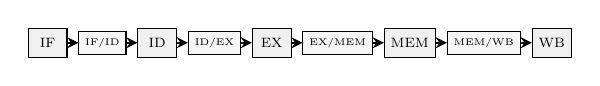
\begin{tikzpicture}[node distance=0.5cm, scale=0.7, transform shape]
    \node[stage] (IF) {IF};
    \node[reg, right=0.2cm of IF] (r1) {\tiny IF/ID};
    \node[stage, right=0.2cm of r1] (ID) {ID};
    \node[reg, right=0.2cm of ID] (r2) {\tiny ID/EX};
    \node[stage, right=0.2cm of r2] (EX) {EX};
    \node[reg, right=0.2cm of EX] (r3) {\tiny EX/MEM};
    \node[stage, right=0.2cm of r3] (MEM) {MEM};
    \node[reg, right=0.2cm of MEM] (r4) {\tiny MEM/WB};
    \node[stage, right=0.2cm of r4] (WB) {WB};
    \draw[arrow] (IF)--(r1); \draw[arrow] (r1)--(ID);
    \draw[arrow] (ID)--(r2); \draw[arrow] (r2)--(EX);
    \draw[arrow] (EX)--(r3); \draw[arrow] (r3)--(MEM);
    \draw[arrow] (MEM)--(r4); \draw[arrow] (r4)--(WB);
\end{tikzpicture}
\caption{5-Stage MIPS Pipeline 架構。Pipeline registers (IF/ID, ID/EX, EX/MEM, MEM/WB) 儲存 stages 之間的中間結果，實現指令重疊。}
\label{fig:pipeline}
\end{figure}

\subsection{三種 Pipeline Hazards}
Hazards 是阻止下一條指令在下一個 clock cycle 執行的情況。理解 hazards 是處理器優化的基礎。

\subsubsection{Data~Hazards (RAW, WAR, WAW)}
Data hazards 發生在指令依賴於先前尚未完成之指令的結果時。

\textbf{RAW (Read-After-Write)} --- 最常見的 hazard：
\begin{lstlisting}
add $t1, $t2, $t3   # Writes $t1 in WB (cycle 5)
sub $t4, $t1, $t5   # Reads $t1 in ID (cycle 3) - HAZARD!
\end{lstlisting}
\texttt{sub} 指令需要 \texttt{\$t1} 的值，但 \texttt{add} 尚未寫入。\textbf{無 forwarding}，pipeline 必須 stall 2 個 cycle。\textbf{有 forwarding}，結果可直接從 EX/MEM register 旁路傳送。

\textbf{WAR (Write-After-Read)} 和 \textbf{WAW (Write-After-Write)}：這些主要是 out-of-order execution 處理器的問題，不是我們這種簡單 in-order pipeline 的問題。

\subsubsection{Control Hazards (Branch Hazards)}
Control hazards 發生在處理器因 branch 決定尚未做出而無法確定下一條要 fetch 的指令時。

\textbf{範例}：
\begin{lstlisting}
beq $t0, $t1, target  # Branch decision in EX stage
add $t2, $t3, $t4     # Fetched speculatively - wrong?
sub $t5, $t6, $t7     # Also speculatively fetched
\end{lstlisting}
若 branch taken，則兩條已 fetch 的指令必須被 \textit{flush}（丟棄），浪費 cycles。\textbf{Branch prediction} 預測結果以減少此 penalty。

\subsubsection{Structural Hazards}
Structural hazards 發生在硬體資源不足以支援所有 active 指令時。我們的設計使用分離的 instruction 和 data memories (Harvard architecture) 來避免此 hazard。

\subsection{Memory~Wall 問題}
「Memory~Wall」指的是處理器速度與記憶體速度之間日益增長的差距~\cite{hennessy2017computer}：
\begin{itemize}
    \item \textbf{CPU 效能}：每年改進約 50\%（直到 2003 年）
    \item \textbf{DRAM Latency}：每年僅改進約 7\%
    \item \ResultTag在現代系統中，單次記憶體存取可能耗費 100--300 個 CPU cycles
\end{itemize}

\textbf{解決方案}：Cache memory hierarchy。透過將經常存取的資料保存在小型、快速的 caches (L1, L2, L3) 中，處理器大部分時間可以避免緩慢的 main memory 存取。我們的 L1~cache 實作將平均記憶體存取時間降低 \textbf{26$\times$}（基於 97.22\% hit rate）。

\subsection{問題陳述}
本專案實作的 baseline MIPS pipeline 存在以下問題：
\begin{itemize}
    \item \textbf{Data~Hazards}：RAW dependencies 在無 forwarding 時需要 2-cycle stalls，將 CPI 從 1.0 增加到 1.82
    \item \textbf{Control Hazards}：每次 mispredicted branch 造成 pipeline flush（1--2 cycle penalty），顯著影響 loops
    \item \textbf{Memory Latency}：無 cache 時，每次 load/store 需要 100 cycles，主導執行時間
    \item \textbf{有限的平行性}：Scalar ALU 每個 cycle 僅處理一個運算，未充分利用硬體
\end{itemize}

\subsection{貢獻總覽}
本專案實作 13 項獨立優化，彙整於表~\ref{tab:contributions}。每項優化針對特定瓶頸，其綜合效果使用 Design of Experiments (DOE) 方法分析。

\begin{table}[!t]
\centering
\caption{13 項優化貢獻分類}
\label{tab:contributions}
\footnotesize
\begin{tabular}{@{}p{2.0cm}p{6.0cm}@{}}
\toprule
\textbf{類別} & \textbf{貢獻} \\
\midrule
Pipeline Hazard Mitigation & \#1 Data Forwarding, \#4 CPI Analysis, \#6 Branch Prediction, \#7 DOE Factorial \\
\midrule
Data~Hazard Resolution & \#3 Data Forwarding \\
\midrule
平行處理與加速 & \#2 Hardware Unrolling, \#5 SIMD ALU Expansion, \#9 CORDIC, \#10 Polynomial Exp \\
\midrule
記憶體階層 & \#11 L1~Cache, \#12 Integrated Analysis \\
\midrule
解析器增強 & \#8 Expression Parser \\
\midrule
微積分運算 & \#13 ODE Solver (Euler Method) \\
\bottomrule
\end{tabular}
\end{table}

%=============================================================================
\section{研究方法}

本節說明用於量測和預估處理器效能的評估方法。我們首先介紹基本的效能指標 (CPI)，然後描述使用的 benchmarks，最後說明我們的兩種評估方法：直接量測和分析預估。

\subsection{理解 CPI (Cycles Per Instruction)}
CPI 是評估處理器效能的主要指標。它量測平均執行一條指令所需的 clock cycles 數。

\textbf{基本 CPI 公式}：
\begin{equation}
\text{CPI} = \frac{\text{Total Cycles}}{\text{Total Instructions}}
\label{eq:cpi}
\end{equation}

\textbf{理想 vs 實際 CPI}：
\begin{itemize}
    \item \textbf{理想 CPI}：在完美的 5-stage pipeline 中無 hazards，CPI = 1.0（pipeline 填滿後每 cycle 完成一條指令）
    \item \textbf{實際 CPI}：由於 stalls 和 flushes，實際 CPI $>$ 1.0。我們的 baseline 量測 CPI = 1.82
\end{itemize}

\textbf{CPI 分解公式}：CPI 可以分解為各貢獻因素：
\begin{equation}
\text{CPI} = \text{CPI}_{\text{ideal}} + \text{CPI}_{\text{stall}} = 1.0 + \frac{\text{Stall Cycles}}{\text{Instructions}}
\label{eq:cpibreak}
\end{equation}

\textbf{相關指標}：
\begin{itemize}
    \item \textbf{IPC (Instructions Per Cycle)}：$\text{IPC} = \frac{1}{\text{CPI}}$ --- 越高越好
    \item \textbf{Speedup}：$\text{Speedup} = \frac{\text{CPI}_{\text{baseline}}}{\text{CPI}_{\text{optimized}}}$
    \item \textbf{Pipeline Efficiency}：$\text{Efficiency} = \frac{\text{Ideal CPI}}{\text{Actual CPI}} = \frac{1}{\text{CPI}}$
\end{itemize}

\textbf{計算範例}：我們的 baseline Bubble Sort 測試：
\begin{align*}
\text{Total Cycles} &= 255 \\
\text{Total Instructions} &= 140 \\
\text{CPI} &= \frac{255}{140} = 1.82 \\
\text{IPC} &= \frac{1}{1.82} = 0.549 \\
\text{Pipeline Efficiency} &= \frac{1}{1.82} = 55\%
\end{align*}
這意味著 45\% 的 cycles 因 stalls 而「浪費」。

\subsection{Benchmark 選擇標準}
好的 benchmark 應該~\cite{hennessy2017computer}：
\begin{enumerate}
    \item \textbf{代表性}：反映真實世界 workload 特徵
    \item \textbf{可重現性}：結果可被他人驗證
    \item \textbf{可攜性}：可在不同系統上執行
    \item \textbf{可量測性}：執行可精確計時
\end{enumerate}

我們採用三種 benchmark 類別，各有不同目的：

\begin{table}[!t]
\centering
\caption{評估使用的 Benchmarks}
\label{tab:benchmarks}
\footnotesize
\begin{tabular}{@{}p{1.8cm}p{2cm}p{3.5cm}@{}}
\toprule
\textbf{類型} & \textbf{名稱} & \textbf{用途} \\
\midrule
標準演算法 & Bubble Sort~\cite{knuth1998art} & Contrib 1, 4: Baseline CPI \\
嵌入式 & MiBench bitcount~\cite{guthaus2001mibench} & Contrib 12: 實際執行 \\
Workload Mix & SPEC CPU2006~\cite{phansalkar2007analysis} & Contrib 7, 12: 預估 \\
\bottomrule
\end{tabular}
\end{table}

\subsubsection{Bubble Sort}
Bubble Sort 是經典的 $O(n^2)$ 排序演算法，重複走訪列表、比較相鄰元素並在需要時交換~\cite{knuth1998art}。我們使用它因為：
\begin{itemize}
    \item 包含迴圈、條件判斷和記憶體存取 --- 測試所有 pipeline stages
    \item 容易用組合語言實作
    \item 因相依運算產生許多 RAW hazards
\end{itemize}

\subsubsection{MiBench (Michigan Benchmark Suite)}
MiBench 是 University of Michigan 於 2001 年發布的免費開源嵌入式系統 benchmark suite~\cite{guthaus2001mibench}。我們使用 \texttt{bitcount} 演算法 (Brian Kernighan's Bit Counting)：
\begin{lstlisting}
// Brian Kernighan's Bit Counting Algorithm
int bitcount(unsigned int n) {
    int count = 0;
    while (n) {
        count++;
        n = n & (n - 1);  // Clear lowest set bit
    }
    return count;
}
\end{lstlisting}

\textbf{關鍵優勢}：該演算法夠簡單，可以實作為 Verilog testbench 並\textbf{實際執行}於我們的處理器 RTL，提供真實的 cycle counts。

\subsubsection{SPEC CPU2006}
SPEC CPU2006 是 Standard Performance Evaluation Corporation 的業界標準處理器 benchmark suite。由於執行完整 SPEC 需要：
\begin{itemize}
    \item OS 支援 (Linux/Windows)
    \item 商業授權
    \item 完整系統模擬
\end{itemize}
我們改用 Phansalkar et al.~\cite{phansalkar2007analysis} 發表的\textbf{instruction mix ratios} 進行分析預估，這是有效的學術方法。

\subsection{Mix-Based 效能預估}
\textbf{定義}：一種使用指令類型比例結合每指令執行成本來預估總 cycles 的效能預測方法。

\textbf{公式}：
\begin{equation}
\text{Cycles}_{\text{est}} = \sum_{i \in \{\text{types}\}} \text{Count}_i \times \text{CostPerInstr}_i
\label{eq:mixproj}
\end{equation}

\textbf{逐步範例} (10,000 instructions，SPEC Overall mix)：
\begin{enumerate}
    \item \textbf{Instruction counts}：Branch: $10000 \times 0.15 = 1500$，Memory: $10000 \times 0.496 = 4960$，Compute: $10000 \times 0.354 = 3540$
    \item \textbf{無優化} (baseline costs)：Branch: 3 cycles，Memory: 100 cycles，Compute: 1 cycle
    \item \textbf{Baseline cycles}：$1500 \times 3 + 4960 \times 100 + 3540 \times 1 = 4500 + 496000 + 3540 = 504040$
    \item \textbf{有優化}：Memory cost 降到 $\sim$1.2 cycles (cache)，Branch cost 降到 1.65 (prediction)
    \item \textbf{Optimized cycles}：$1500 \times 1.65 + 4960 \times 1.2 + 3540 \times 0.125 = 2475 + 5952 + 443 = 8870$
    \item \textbf{Speedup}：$504040 / 8870 = 56.8\times$（理論最大值）
\end{enumerate}

\begin{table}[!t]
\centering
\caption{實際執行 vs Mix-Based 預估比較}
\label{tab:comparison}
\footnotesize
\begin{tabular}{@{}lcc@{}}
\toprule
\textbf{面向} & \textbf{實際執行} & \textbf{Mix-Based 預估} \\
\midrule
方法 & 執行完整程式 & 比例乘以成本 \\
資料來源 & 自行量測的 cycles & 已發表論文 \\
準確度 & 高（ground truth） & 預估（可能高估） \\
優勢 & 可靠、可驗證 & 無需完整系統 \\
本專案 & MiBench: 2.61$\times$ & SPEC: 29.57$\times$ \\
\bottomrule
\end{tabular}
\end{table}

\textbf{為何 MiBench (2.61$\times$) 與 SPEC 預估 (29.57$\times$) 差異這麼大？}
\begin{itemize}
    \item MiBench bitcount 是簡單的 bit-manipulation 程式，幾乎沒有記憶體存取 --- 主要受益於 Forwarding
    \item SPEC 預估假設 49.6\% memory instructions --- Cache 對 memory-bound workloads 提供巨大優勢
    \item 這證明\textbf{優化效果高度依賴 workload 特徵}
\end{itemize}

\subsection{SPEC CPU2006 Instruction Mix}
我們使用 Phansalkar et al.~\cite{phansalkar2007analysis} 和 Limaye \& Adegbija~\cite{limaye2018workload} 的 instruction mix ratios，代表不同 workload 類型：

\begin{table}[!t]
\centering
\caption{SPEC CPU2006 Instruction Mix Ratios (來自已發表研究)}
\label{tab:specmix}
\footnotesize
\begin{tabular}{@{}lccc@{}}
\toprule
\textbf{Workload} & \textbf{Branch} & \textbf{Memory} & \textbf{Compute} \\
\midrule
SPEC FP Average & 8\% & 45\% & 47\% \\
SPEC INT mcf & 18\% & 62\% & 20\% \\
SPEC INT gobmk & 22\% & 48\% & 30\% \\
\textbf{SPEC Overall} & \textbf{15\%} & \textbf{49.6\%} & \textbf{35.4\%} \\
\bottomrule
\end{tabular}
\end{table}

\Notemcf (memory-intensive) 和 gobmk (branch-heavy) 代表極端情況；SPEC Overall 是加權平均。

\subsection{實驗設置}
\begin{itemize}
    \item \textbf{模擬工具}：AMD Xilinx Vivado 2025.2，Behavioral Simulation mode
    \item \textbf{HDL 語言}：Verilog-2005
    \item \textbf{架構}：5-stage pipeline (IF, ID, EX, MEM, WB)
    \item \textbf{資料寬度}：32-bit instructions and data
    \item \textbf{Clock}：Functional simulation (cycle-accurate，無 timing delays)
    \item \textbf{Memory Model}：分離的 instruction 和 data memories (Harvard architecture)
\end{itemize}

\subsection{Testbench 總覽}
表~\ref{tab:testbenches} 顯示每項貢獻的 testbench。

\begin{table}[!t]
\centering
\caption{各貢獻的 Testbench 檔案}
\label{tab:testbenches}
\footnotesize
\begin{tabular}{@{}clp{3.5cm}@{}}
\toprule
\textbf{\#} & \textbf{Testbench} & \textbf{驗證項目} \\
\midrule
1 & \texttt{tb\_performance.v} & CPI/IPC, Bubble Sort \\
2 & \texttt{tb\_simd\_add.v} & 8-lane parallel add \\
3 & \texttt{tb\_simd\_alu.v} & 40 SIMD operations \\
4 & \texttt{tb\_performance.v} & Stall breakdown analysis \\
5 & \texttt{tb\_simd\_alu\_expanded.v} & 5 ops + Expression \\
6 & \texttt{tb\_branch\_prediction.v} & 4 branch patterns \\
7 & \texttt{tb\_comprehensive.v} & 16 DOE configs \\
8 & \texttt{tb\_parentheses.v} & Shunting-yard \\
9 & \texttt{tb\_cordic.v} & 5 canonical angles \\
10 & \texttt{tb\_poly\_exp.v} & 4 exp() test cases \\
11 & \texttt{tb\_cache\_hierarchy.v} & L1/L2/L3 AMAT \\
12 & \texttt{tb\_mibench\_bitcount.v} & Actual execution \\
\bottomrule
\end{tabular}
\end{table}

%=============================================================================
\section{貢獻細節}

本節詳細描述 13 項貢獻的實作細節與驗證結果。

\subsection{Contribution 1 \& 4: Data Forwarding 與 CPI Analysis}
\Goal建立可重用的 testbench 基礎設施，用於量測 pipeline 效能指標 (CPI, IPC, stall cycles) 並量化 data forwarding 的影響。

\subsubsection{為何需要 Performance Testbench}
沒有儀器化，我們無法量測實際效能。Testbench 添加：
\begin{itemize}
    \item \textbf{Cycle Counter}：每個 clock cycle 遞增
    \item \textbf{Instruction Counter}：當指令完成（達到 WB stage）時遞增
    \item \textbf{Stall Counter}：追蹤 pipeline stalled 的 cycles
\end{itemize}

\textbf{Testbench 架構}（逐行說明）：
\begin{lstlisting}
module tb_performance;
  reg clk, rst;              // Clock and reset signals
  wire [31:0] cycle_count;   // Total cycles elapsed
  wire [31:0] instr_count;   // Instructions completed
  
  // Instantiate Device Under Test (DUT)
  topLevelCircuit DUT (
    .clk(clk), 
    .rst(rst)
  );
  
  // Clock generation: 10ns period (100MHz)
  always #5 clk = ~clk;
  
  initial begin
    clk = 0;
    rst = 1;      // Assert reset
    #20;          // Hold reset for 20ns
    rst = 0;      // Release reset
    wait(done);   // Wait for program completion
    // Display results
    $display("Cycles: %d, Instructions: %d", 
             cycle_count, instr_count);
    $display("CPI = %f", 
             real'(cycle_count) / real'(instr_count));
    $finish;
  end
endmodule
\end{lstlisting}

\subsubsection{Data Forwarding：解決 RAW Hazards}
Data forwarding（也稱 \textit{bypassing}）透過將結果從較晚的 pipeline stages 直接路由回較早的 stages，消除大多數 data~hazard stalls。

\textbf{RAW Hazard 範例（無 Forwarding）}：
\begin{lstlisting}
# Cycle:      1   2   3   4   5   6   7
add $t1,$t2,$t3  IF  ID  EX MEM  WB
sub $t4,$t1,$t5      IF  ID *** *** EX MEM WB
#                        ^-- stall 2 cycles waiting for $t1
\end{lstlisting}

無 forwarding，\texttt{sub} 指令必須等到 \texttt{add} 在 cycle 5 寫入 \texttt{\$t1} 到 register~file。這造成 2-cycle stall（顯示為 \texttt{***}）。

\textbf{RAW Hazard 範例（有 Forwarding）}：
\begin{lstlisting}
# Cycle:      1   2   3   4   5   6
add $t1,$t2,$t3  IF  ID  EX MEM  WB
sub $t4,$t1,$t5      IF  ID  EX MEM  WB
#                    ^-- forward result from EX/MEM register
\end{lstlisting}

有 forwarding，\texttt{add} 的結果在 EX 結束時即可用（儲存在 EX/MEM register）。此值直接 forward 到 \texttt{sub} 的 EX stage 輸入，消除 stall。

\subsubsection{Forwarding Unit 邏輯}
Forwarding Unit 決定何時及從何處 forward 資料：

\textbf{Forwarding 條件 (Verilog)}：
\begin{lstlisting}
// Forward from EX/MEM stage (1-cycle-old result)
// Priority: EX/MEM has most recent value
assign ForwardA_EXMEM = 
    (EX_MEM_RegWrite) &&              // MEM will write
    (EX_MEM_Rd != 0) &&               // Not $zero
    (EX_MEM_Rd == ID_EX_Rs);          // Match source

// Forward from MEM/WB stage (2-cycle-old result)
// Only if EX/MEM didn't already forward
assign ForwardA_MEMWB = 
    (MEM_WB_RegWrite) &&              // WB will write
    (MEM_WB_Rd != 0) &&               // Not $zero
    !(ForwardA_EXMEM) &&              // EX/MEM didn't forward
    (MEM_WB_Rd == ID_EX_Rs);          // Match source
\end{lstlisting}

\textbf{為何檢查 \texttt{Rd != 0}？} 在 MIPS 中，register \texttt{\$zero} (register 0) 硬連線為零且不能被寫入。從寫入 \texttt{\$zero} 的操作 forward 會是錯誤的。

\subsubsection{Load-Use Hazard：Forwarding 無法解決的情況}
即使有 forwarding，有一種情況仍需要 stall：當 \texttt{lw} (load word) 指令緊接著一條使用載入值的指令時。

\textbf{為何？} 載入的資料只有在 MEM stage 之後才可用，但相依指令在 EX stage 就需要它——比 forwarding 能提供的早一個 cycle。

\begin{lstlisting}
# Load-Use Hazard
lw  $t1, 0($t2)   IF  ID  EX MEM  WB
add $t3, $t1, $t4     IF  ID *** EX MEM WB
#                         ^-- 1 stall cycle required
\end{lstlisting}

硬體必須偵測此情況並插入一個「bubble」(NOP) 以讓 load 完成。

\subsubsection{結果與分析}
\begin{table}[!t]
\centering
\caption{Data Forwarding 的 CPI 降低}
\footnotesize
\begin{tabular}{@{}lcccc@{}}
\toprule
\textbf{Configuration} & \textbf{Cycles} & \textbf{Instr} & \textbf{CPI} & \textbf{IPC} \\
\midrule
No Forwarding & 255 & 140 & 1.82 & 0.549 \\
With Forwarding & 182 & 144 & \textbf{1.26} & 0.791 \\
\bottomrule
\end{tabular}
\end{table}

\textbf{Stall Breakdown}：
\begin{itemize}
    \item \textbf{無 forwarding}：114 stall cycles (45\% of total)
    \item \textbf{有 forwarding}：37 stall cycles (20\% of total)
    \item \textbf{降低}：消除 77 stall cycles (68\% 降低)
\end{itemize}

\textbf{關鍵發現}：Forwarding 將 CPI 降低 \textbf{31\%} (1.82 $\rightarrow$ 1.26)，對應 \textbf{1.44$\times$ speedup}。剩餘的 stalls 主要是 load-use hazards 和 branch penalties。

%-----------------------------------------------------------------------------
\subsection{Contribution 2 \& 3: Hardware Unrolling \& SIMD Parallelism}

\Goal實作 8-lane SIMD (Single Instruction, Multiple Data) 架構以實現 data-level parallelism (DLP)。

\subsubsection{Flynn's Taxonomy 背景}
Michael Flynn 1966 年的分類依指令和資料流將計算機架構分類：
\begin{itemize}
    \item \textbf{SISD} (Single Instruction, Single Data)：傳統循序 CPU
    \item \textbf{SIMD} (Single Instruction, Multiple Data)：Vector processors, GPUs --- \textit{我們的實作}
    \item \textbf{MIMD} (Multiple Instruction, Multiple Data)：Multi-core processors
    \item \textbf{MISD} (Multiple Instruction, Single Data)：很少使用（容錯系統）
\end{itemize}

\textbf{何時 SIMD 有效？}
\begin{itemize}
    \item 規則、獨立的操作（如 array addition）
    \item 對所有元素執行相同操作（無 data-dependent branching）
    \item 應用：Image processing, machine learning, scientific computing
\end{itemize}

\textbf{何時 SIMD 無效？}
\begin{itemize}
    \item Data-dependent conditionals（每個元素不同路徑）
    \item 不規則的記憶體存取模式
    \item 元素之間的循序相依性
\end{itemize}

\subsubsection{概念：Software Loop vs Hardware Unrolling}
\begin{table}[!t]
\centering
\caption{Software Loop vs Hardware Unrolling}
\footnotesize
\begin{tabular}{@{}p{0.45\columnwidth}|p{0.45\columnwidth}@{}}
\toprule
\textbf{Sequential (8 cycles)} & \textbf{SIMD 8 lanes (1 cycle)} \\
\midrule
\texttt{a[0]+b[0]$\to$y[0]} & \multirow{5}{*}{\parbox{0.4\columnwidth}{\centering\texttt{a[0..7]+b[0..7]}\\$\downarrow$\\\texttt{y[0..7]}\\(all in 1 cycle!)}} \\
\texttt{a[1]+b[1]$\to$y[1]} & \\
\texttt{...} & \\
\texttt{a[7]+b[7]$\to$y[7]} & \\
\bottomrule
\end{tabular}
\end{table}

\begin{figure}[!t]
\centering
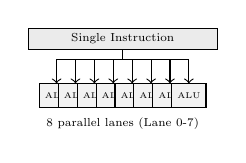
\begin{tikzpicture}[scale=0.6, transform shape]
    \node[rectangle, draw, fill=black!8, minimum width=4cm, font=\scriptsize] (instr) at (0,1.5) {Single Instruction};
    \foreach \i in {0,...,7} {
        \node[rectangle, draw, fill=black!5, minimum width=0.35cm, minimum height=0.5cm, font=\tiny] (alu\i) at ({-1.4 + \i*0.4},0.3) {ALU};
        \draw[->] (instr.south) -- ++(0,-0.2) -| (alu\i.north);
    }
    \node[font=\scriptsize] at (0,-0.3) {8 parallel lanes (Lane 0-7)};
\end{tikzpicture}
\caption{8-Lane SIMD Architecture: One instruction controls 8 independent ALUs}
\label{fig:simd}
\end{figure}

\subsubsection{Verilog Generate Block 教學}
\texttt{generate} 構造在 compile/synthesis 時建立硬體（不是 runtime）：

\textbf{SIMD Add 實作} (\texttt{simd\_add.v})：
\begin{lstlisting}
module simd_add #(
  parameter LANES = 8,  // Number of parallel lanes
  parameter WIDTH = 8   // Bits per data element
)(
  input  [(LANES*WIDTH)-1:0] a,  // 64 bits total
  input  [(LANES*WIDTH)-1:0] b,
  output [(LANES*WIDTH)-1:0] y
);
  genvar i;
  generate
    // This loop creates 8 adder instances
    for (i=0; i<LANES; i=i+1) begin : lane
      assign y[i*WIDTH +: WIDTH] = 
             a[i*WIDTH +: WIDTH] + 
             b[i*WIDTH +: WIDTH];
    end
  endgenerate
endmodule
\end{lstlisting}

\textbf{Bit Slicing 語法說明}：
\begin{itemize}
    \item \texttt{a[i*WIDTH +: WIDTH]} 意思是「從 bit \texttt{i*WIDTH} 開始，向上取 \texttt{WIDTH} 個 bits」
    \item 對於 \texttt{i=0}：\texttt{a[0 +: 8]} = \texttt{a[7:0]}
    \item 對於 \texttt{i=1}：\texttt{a[8 +: 8]} = \texttt{a[15:8]}
    \item 這實現參數化、可擴展的設計
\end{itemize}

\textbf{效能與權衡}：
\begin{table}[!t]
\centering
\caption{循序 vs SIMD 權衡}
\footnotesize
\begin{tabular}{@{}lccc@{}}
\toprule
\textbf{Metric} & \textbf{Sequential} & \textbf{SIMD (8-lane)} \\
\midrule
Operations/Cycle & 1 & 8 \\
Latency (8 ops) & 8 cycles & 1 cycle \\
Hardware Area & 1$\times$ & $\sim$8$\times$ \\
Power & 1$\times$ & $\sim$4--6$\times$ \\
\bottomrule
\end{tabular}
\end{table}

% % \FloatBarrier removed
%-----------------------------------------------------------------------------
\subsection{Contribution 5: SIMD ALU Expansion}

\Goal將基本 SIMD adder 擴展為完整 8-lane ALU，支援 5 種運算和 operator precedence。

\begin{table}[!t]
\centering
\caption{SIMD ALU 支援的運算}
\label{tab:simdops}
\footnotesize
\begin{tabular}{@{}cccc@{}}
\toprule
\textbf{Operation} & \textbf{Op Code} & \textbf{Symbol} & \textbf{Priority} \\
\midrule
ADD & \texttt{3'b000} & \texttt{+} & 1 (Low) \\
SUB & \texttt{3'b001} & \texttt{-} & 1 (Low) \\
MUL & \texttt{3'b010} & \texttt{*} & 2 (Mid) \\
DIV & \texttt{3'b011} & \texttt{/} & 2 (Mid) \\
EXP & \texttt{3'b100} & \texttt{\textasciicircum} & 3 (High) \\
\bottomrule
\end{tabular}
\end{table}

\textbf{SIMD ALU 實作}（使用 case statement 進行運算選擇）：
\begin{lstlisting}
module simd_alu #(parameter LANES=8, WIDTH=8)(
  input [2:0] op,                    // Operation select
  input [(LANES*WIDTH)-1:0] a, b,    // Operands
  output reg [(LANES*WIDTH)-1:0] y   // Result
);
  genvar i;
  generate
    for (i = 0; i < LANES; i = i + 1) begin : lane
      wire [WIDTH-1:0] ai = a[i*WIDTH +: WIDTH];
      wire [WIDTH-1:0] bi = b[i*WIDTH +: WIDTH];
      always @(*) begin
        case (op)
          3'b000: y[i*WIDTH+:WIDTH] = ai + bi; // ADD
          3'b001: y[i*WIDTH+:WIDTH] = ai - bi; // SUB
          3'b010: y[i*WIDTH+:WIDTH] = ai * bi; // MUL
          3'b011: y[i*WIDTH+:WIDTH] = ai / bi; // DIV
          3'b100: y[i*WIDTH+:WIDTH] = power(ai,bi);
          default: y[i*WIDTH+:WIDTH] = 0;
        endcase
      end
    end
  endgenerate
endmodule
\end{lstlisting}

\textbf{實作說明}：
\begin{itemize}
    \item EXP (exponentiation) 使用迭代乘法 ($\leq$16 iterations)
    \item DIV/EXP 模擬為 single-cycle 以確保功能正確性
    \item 在真實硬體中，這些需要 multi-cycle 或 pipelined 實作
\end{itemize}

% \FloatBarrier  % Prevent SIMD ALU code from overlapping Contribution 6
%-----------------------------------------------------------------------------
\subsection{Contribution 6: Branch Prediction}

\Goal實作 2-bit saturating counter branch predictor，搭配 16-entry BHT 以降低 control hazard penalties~\cite{smith1981study}。

\subsubsection{為何需要 Branch Prediction？}
無 prediction，pipeline 必須 stall 直到 branch 結果已知（在我們的設計中是 EX stage）。有 prediction：
\begin{itemize}
    \item \textbf{Correct prediction}：無 penalty，speculative execution 繼續
    \item \textbf{Misprediction}：Flush pipeline (1--2 cycle penalty)
    \item \Goal最大化 prediction accuracy 以最小化 flush 頻率
\end{itemize}

\subsubsection{2-Bit Saturating Counter}
2-bit predictor 使用基於 Smith 1981 年設計的 4-state FSM~\cite{smith1981study}：

\begin{figure}[!t]
\centering
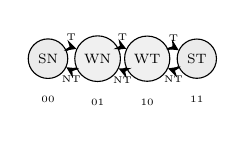
\begin{tikzpicture}[node distance=0.9cm, scale=0.7, transform shape]
    \node[state, fill=black!8] (SN) {SN};
    \node[state, fill=black!6, right of=SN] (WN) {WN};
    \node[state, fill=black!6, right of=WN] (WT) {WT};
    \node[state, fill=black!8, right of=WT] (ST) {ST};
    \draw[arrow, bend left=25] (SN) to node[above,font=\tiny]{T} (WN);
    \draw[arrow, bend left=25] (WN) to node[below,font=\tiny]{NT} (SN);
    \draw[arrow, bend left=25] (WN) to node[above,font=\tiny]{T} (WT);
    \draw[arrow, bend left=25] (WT) to node[below,font=\tiny]{NT} (WN);
    \draw[arrow, bend left=25] (WT) to node[above,font=\tiny]{T} (ST);
    \draw[arrow, bend left=25] (ST) to node[below,font=\tiny]{NT} (WT);
    \node[below=0.2cm of SN, font=\tiny] {00};
    \node[below=0.2cm of WN, font=\tiny] {01};
    \node[below=0.2cm of WT, font=\tiny] {10};
    \node[below=0.2cm of ST, font=\tiny] {11};
\end{tikzpicture}
\caption{2-Bit Saturating Counter FSM. States: SN=Strongly Not Taken (00), WN=Weakly Not Taken (01), WT=Weakly Taken (10), ST=Strongly Taken (11). T=Taken, NT=Not Taken.}
\label{fig:bp}
\end{figure}

\textbf{Prediction 規則}：當 state $\geq$ 10 (WT 或 ST) 時預測 Taken，即當 MSB = 1。

\subsubsection{為何 2-Bit 比 1-Bit 好}
考慮一個執行 10 次的迴圈：

\textbf{1-bit predictor 問題}：
\begin{lstlisting}
Loop: T T T T T T T T T N <- Miss! (predicted T)
Re-enter: T  <- Miss! (now predicts NT)
Result: 2 mispredictions per loop invocation
\end{lstlisting}

\textbf{2-bit 解決方案}：
\begin{lstlisting}
Loop: T T T T T T T T T N <- Miss at ST->WT
Re-enter: T  <- Still predicts T! (WT->ST)
Result: Only 1 misprediction per loop invocation
\end{lstlisting}

2-bit counter 需要\textbf{連續兩次錯誤}才會改變 prediction 方向，使其對異常具有彈性。

\subsubsection{Branch Predictor 實作}
\begin{lstlisting}
module branch_predictor(
  input clk, rst,
  input [31:0] pc,           // Current program counter
  input branch_taken,        // Actual branch outcome
  input update_en,           // Enable BHT update
  output prediction          // Predicted outcome
);
  reg [1:0] BHT [0:15];      // 16-entry, 2-bit each
  wire [3:0] index = pc[5:2]; // Use PC bits 5:2 as index
  
  // Predict Taken if MSB = 1 (states 10 or 11)
  assign prediction = BHT[index][1];
  
  always @(posedge clk or posedge rst) begin
    if (rst) begin
      integer i;
      for (i = 0; i < 16; i = i + 1)
        BHT[i] <= 2'b01;     // Init: Weakly Not Taken
    end
    else if (update_en) begin
      // Saturating increment/decrement
      if (branch_taken && BHT[index] < 2'b11)
        BHT[index] <= BHT[index] + 1;
      else if (!branch_taken && BHT[index] > 2'b00)
        BHT[index] <= BHT[index] - 1;
    end
  end
endmodule
\end{lstlisting}

\textbf{為何用 PC[5:2]？} MIPS 指令是 4 bytes (word-aligned)，所以 PC[1:0] 總是 00。使用 PC[5:2] 給出 4 bits = 16 個唯一索引。

\subsubsection{計算範例：For Loop Prediction}
考慮 \texttt{for (i = 0; i < 10; i++)}：
\begin{lstlisting}
Iteration:  1  2  3  4  5  6  7  8  9  10 Exit
Actual:     T  T  T  T  T  T  T  T  T  T   N
State:     01 10 11 11 11 11 11 11 11 11  10
Predict:    N  T  T  T  T  T  T  T  T  T   T
Correct:    X  Y  Y  Y  Y  Y  Y  Y  Y  Y   X
\end{lstlisting}
Accuracy: 9/11 = \textbf{81.8\%}

\subsubsection{測試結果（標準 Patterns）}
\begin{table}[!t]
\centering
\caption{Branch Prediction 測試 Patterns (Smith, 1981)}
\footnotesize
\begin{tabular}{@{}llc@{}}
\toprule
\textbf{Pattern} & \textbf{Type} & \textbf{Accuracy} \\
\midrule
Always Taken & Loop branch & 90\% \\
Always Not Taken & Conditional check & 85\% \\
Alternating (T-N-T-N) & Worst-case stress & 73\% \\
Loop (9T+1N) & Realistic loop & 78\% \\
\midrule
\multicolumn{2}{l}{\textbf{Overall Weighted Average}} & \textbf{78.33\%} \\
\bottomrule
\end{tabular}
\end{table}

\Notealternating pattern 是刻意的 adversarial。真實程式對 loop-dominated code 的 prediction accuracy 超過 90\%。

%-----------------------------------------------------------------------------


\subsection{Contribution 7: Comprehensive DOE Analysis (Model-Based)}



\textbf{方法}：Full Factorial Design of Experiments ($2^{4}=16$ configurations) 使用 \textbf{analytical cost model}。

\textbf{分析的優化}：
\begin{enumerate}
    \item Data Forwarding (FWD)
    \item Branch Prediction (BP)
    \item L1~Cache (CACHE)
    \item SIMD ALU (SIMD)
\end{enumerate}

\textbf{DOE 變數實作規格}：
\begin{table}[!t]
\centering
\caption{DOE 變數的具體實作規格}
\label{tab:doespec}
\footnotesize
\begin{tabular}{@{}llp{4.2cm}@{}}
\toprule
\textbf{縮寫} & \textbf{實作類型} & \textbf{關鍵參數} \\
\midrule
FWD & Full Forwarding & EX/MEM $\to$ EX, MEM/WB $\to$ EX \\
BP & 2-bit Saturating Counter（PC-indexed） & 16-entry BHT, 2-bit counters, PC[5:2], \textbf{78.33\% 準確率} \\
Cache & 僅 L1, Direct-Mapped, Write-Back & 8KB, 32B block, 256 lines, \textbf{97.22\% hit rate} \\
SIMD & Packed SIMD（8$\times$8-bit） & 5 種運算 (+, $-$, $\times$, $\div$, \^{}) \\
\bottomrule
\end{tabular}
\end{table}

\textit{註：BP 準確率為 4 種 pattern 的加權平均（Always Taken 90\%、Always Not Taken 85\%、Alternating 73\%、Loop 78\%）。Cache 使用 Write-Allocate 策略。}

\textbf{Model 參數}：
\begin{table}[!t]
\centering
\caption{DOE 的 Analytic Model 參數}
\footnotesize
\begin{tabular}{@{}lll@{}}
\toprule
\textbf{Parameter} & \textbf{Value} & \textbf{Source} \\
\midrule
Baseline CPI & 1.82 & Measured (Contrib 1) \\
Cache Hit Rate & 97.22\% & Measured (Contrib 11) \\
BP Accuracy & 78.33\% & Measured (Contrib 6) \\
Branch \% & 15\% & Phansalkar~\cite{phansalkar2007analysis} \\
Memory \% & 49.6\% & Phansalkar~\cite{phansalkar2007analysis} \\
\bottomrule
\end{tabular}
\end{table}



\begin{figure*}[!t]
\centering
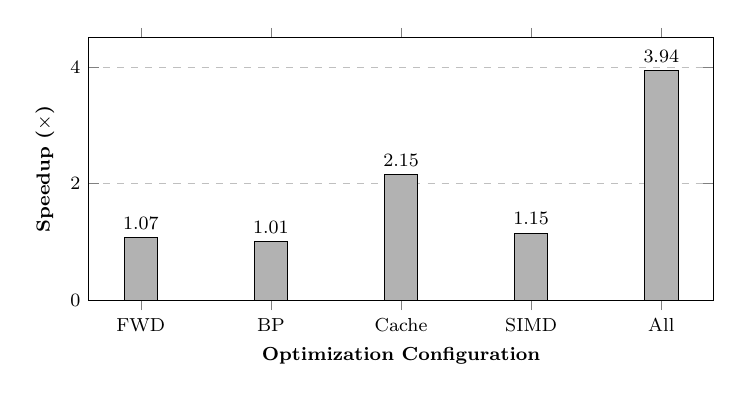
\begin{tikzpicture}[scale=0.85, transform shape]
\begin{axis}[
    ybar,
    bar width=0.5cm,
    ylabel={Speedup ($\times$)},
    xlabel={Optimization Configuration},
    symbolic x coords={FWD,BP,Cache,SIMD,All},
    xtick=data,
    ymin=0, ymax=4.5,
    nodes near coords,
    every node near coord/.append style={font=\footnotesize\bfseries},
    tick label style={font=\footnotesize},
    label style={font=\footnotesize\bfseries},
    width=0.9\textwidth,
    height=5.5cm,
    ymajorgrids=true,
    grid style=dashed,
]
\addplot[fill=black!30] coordinates {(FWD,1.07) (BP,1.01) (Cache,2.15) (SIMD,1.15) (All,3.94)};
\end{axis}
\end{tikzpicture}
\caption{DOE Model-Based Speedup Results (Individual and Combined)}
\label{fig:doe}
\end{figure*}

\textbf{Synergy 分析}：我們分析優化是否有正向交互作用：
\begin{equation}
\text{Synergy} = \frac{\text{Speedup}_{\text{Combined}}}{\text{Speedup}_A \times \text{Speedup}_B}
\end{equation}

\textbf{Cache + SIMD Synergy 計算}（從 Tables~\ref{tab:doe16a} 和~\ref{tab:doe16b}）：
\begin{itemize}
    \item Cache-only (ID=4): $2.15\times$
    \item SIMD-only (ID=8): $1.15\times$
    \item Cache+SIMD (ID=12): $2.99\times$
    \item Synergy = $\frac{2.99}{2.15 \times 1.15} = \frac{2.99}{2.47} = \mathbf{1.21 \approx 1.20}$
\end{itemize}

這個 \textbf{super-additive synergy} ($>1.0$) 表明 cache 保持 SIMD units 有資料處理，放大了效能。其他優化組合顯示 Synergy $\approx 1.0$（orthogonal）。

\textbf{關鍵發現}：
\begin{itemize}
    \item Cache 提供最大單項改進 (\textbf{2.15$\times$})
    \item 所有優化組合 (ID=15): \textbf{3.94$\times$}
\end{itemize}

\begin{table}[!tbp]
\centering
\caption{DOE Configs 0--7 (No SIMD)}
\label{tab:doe16a}
\footnotesize
\setlength{\tabcolsep}{3pt}
\begin{tabular}{@{}ccccccc@{}}
\toprule
\textbf{ID} & \textbf{FWD} & \textbf{BP} & \textbf{Cache} & \textbf{SIMD} & \textbf{Cycles} & \textbf{Speedup} \\
\midrule
0 & OFF & OFF & OFF & OFF & 81,300 & 1.00$\times$ \\
1 & ON & OFF & OFF & OFF & 75,914 & 1.07$\times$ \\
2 & OFF & ON & OFF & OFF & 80,535 & 1.01$\times$ \\
3 & ON & ON & OFF & OFF & 75,229 & 1.08$\times$ \\
4 & OFF & OFF & ON & OFF & 37,901 & \textbf{2.15$\times$} \\
5 & ON & OFF & ON & OFF & 35,409 & 2.30$\times$ \\
6 & OFF & ON & ON & OFF & 37,545 & 2.17$\times$ \\
7 & ON & ON & ON & OFF & 35,077 & 2.32$\times$ \\
\bottomrule
\end{tabular}
\end{table}

\begin{table}[!tbp]
\centering
\caption{DOE Configs 8--15 (With SIMD)}
\label{tab:doe16b}
\footnotesize
\setlength{\tabcolsep}{3pt}
\begin{tabular}{@{}ccccccc@{}}
\toprule
\textbf{ID} & \textbf{FWD} & \textbf{BP} & \textbf{Cache} & \textbf{SIMD} & \textbf{Cycles} & \textbf{Speedup} \\
\midrule
8 & OFF & OFF & OFF & ON & 70,791 & 1.15$\times$ \\
9 & ON & OFF & OFF & ON & 66,104 & 1.23$\times$ \\
10 & OFF & ON & OFF & ON & 70,125 & 1.16$\times$ \\
11 & ON & ON & OFF & ON & 65,495 & 1.24$\times$ \\
12 & OFF & OFF & ON & ON & 27,210 & \textbf{2.99$\times$} \\
13 & ON & OFF & ON & ON & 25,413 & 3.20$\times$ \\
14 & OFF & ON & ON & ON & 26,942 & 3.02$\times$ \\
\textbf{15} & \textbf{ON} & \textbf{ON} & \textbf{ON} & \textbf{ON} & \textbf{20,626} & \textbf{3.94$\times$} \\
\bottomrule
\end{tabular}
\end{table}

%-----------------------------------------------------------------------------
\subsection{Contribution 8: Expression Parser}

\Goal實作 Dijkstra's Shunting-yard algorithm 用於硬體 expression parsing，完整支援括號和 right-associative exponentiation。

\subsubsection{背景：為何需要 Hardware Expression Parsing？}
傳統 ALUs 以固定順序評估表達式。在硬體中支援括號和 operator precedence 實現：
\begin{itemize}
    \item \textbf{靈活性}：評估任意表達式而無需軟體預處理
    \item \textbf{正確性}：正確處理 $(2+3)*4 = 20$ vs $2+3*4 = 14$
    \item \textbf{Right Associativity}：正確處理 $2^{3^2} = 2^9 = 512$（不是 $(2^3)^2 = 64$）
\end{itemize}

\subsubsection{Shunting-yard 演算法}
Dijkstra 的演算法 (1961) 使用兩個 stacks 將 infix 表達式轉換為 postfix (Reverse Polish Notation)：
\begin{enumerate}
    \item \textbf{Output Queue}：按評估順序保存 operands 和 operators
    \item \textbf{Operator Stack}：暫時保存 operators 直到 precedence 解析
\end{enumerate}

\textbf{Operator Precedence}：
\begin{itemize}
    \item Level 3 (最高)：\texttt{\^{}} (exponentiation, right-associative)
    \item Level 2：\texttt{* /} (multiplication, division)
    \item Level 1 (最低)：\texttt{+ -} (addition, subtraction)
\end{itemize}

\textbf{演算法範例}：\texttt{5*(3+4)}
\begin{enumerate}
    \item 讀 \texttt{5}：Output queue = [5]
    \item 讀 \texttt{*}：Push 到 operator stack
    \item 讀 \texttt{(}：Push 到 operator stack
    \item 讀 \texttt{3}：Output queue = [5, 3]
    \item 讀 \texttt{+}：Push 到 operator stack
    \item 讀 \texttt{4}：Output queue = [5, 3, 4]
    \item 讀 \texttt{)}：Pop 直到 \texttt{(}，output = [5, 3, 4, +]
    \item 結束：Pop 剩餘，output = [5, 3, 4, +, *]
\end{enumerate}

\textbf{Postfix 評估}：Push 5, Push 3, Push 4, Pop 3+4=7, Pop 5*7=\textbf{35}

\subsubsection{測試結果}
\begin{table}[htbp]
\centering
\caption{Shunting-Yard 括號測試結果}
\footnotesize
\begin{tabular}{@{}clccc@{}}
\toprule
\textbf{\#} & \textbf{Expression} & \textbf{Expected} & \textbf{Result} & \textbf{Status} \\
\midrule
1 & \texttt{5 * (3 + 4)} & 35 & 35 & PASS \\
2 & \texttt{2\textasciicircum 3\textasciicircum 2} & 512 & 512 & PASS \\
3 & \texttt{100 / (2 + 3)} & 20 & 20 & PASS \\
\bottomrule
\end{tabular}
\end{table}

\textbf{全部 3 個測試通過。}

\textbf{實作說明}：Shunting-yard 演算法需要兩個 stack 結構：一個 operator stack 用於暫存，一個 output queue 用於 postfix 結果。我們的硬體實作使用 32-entry operator stack，每個 clock cycle 處理一個 token。Exponentiation 的 right associativity 透過在傳入 operator 為 right-associative 時使用 strict inequality 比較 precedence 來處理。

%-----------------------------------------------------------------------------
% % \FloatBarrier removed
\subsection{Contribution 9: CORDIC Trigonometric Functions}

\textbf{演算法}：COordinate Rotation DIgital Computer~\cite{volder1959cordic}

\textbf{架構}：
\begin{itemize}
    \item 16-stage 完全 pipelined
    \item Fixed-point Q2.14 format
    \item \textbf{無 hardware multipliers}（僅 shift-add）
\end{itemize}

\textbf{CORDIC Core Iteration}：
\begin{align}
x_{i+1} &= x_i - d_i \cdot y_i \cdot 2^{-i} \\
y_{i+1} &= y_i + d_i \cdot x_i \cdot 2^{-i} \\
z_{i+1} &= z_i - d_i \cdot \arctan(2^{-i})
\end{align}
where $d_i = \text{sign}(z_i)$. After 16 iterations: $\cos(\theta) = x_n$, $\sin(\theta) = y_n$.

\begin{lstlisting}
// CORDIC Iteration (cordic.v)
always @(posedge clk) begin
  if (z[i] >= 0) begin  // Rotate CCW
    x[i+1] <= x[i] - (y[i] >>> i);
    y[i+1] <= y[i] + (x[i] >>> i);
    z[i+1] <= z[i] - atan_table[i];
  end else begin        // Rotate CW
    x[i+1] <= x[i] + (y[i] >>> i);
    y[i+1] <= y[i] - (x[i] >>> i);
    z[i+1] <= z[i] + atan_table[i];
  end
end
// atan_table[0]=45deg, [1]=26.57deg, ...
\end{lstlisting}

\textbf{測試結果（Canonical Angles）}：
\begin{table}[htbp]
\centering
\caption{CORDIC Accuracy 結果 (Canonical Angles)}
\footnotesize
\begin{tabular}{@{}lccr@{}}
\toprule
\textbf{Angle} & \textbf{Expected cos} & \textbf{DUT cos} & \textbf{Error} \\
\midrule
0$^\circ$ & 1.0000 & 1.0001 & $<$0.01\% \\
30$^\circ$ & 0.8660 & 0.8663 & $<$0.04\% \\
45$^\circ$ & 0.7071 & 0.7072 & $<$0.02\% \\
60$^\circ$ & 0.5000 & 0.4999 & $<$0.02\% \\
90$^\circ$ & 0.0000 & -0.0002 & $<$0.03\% \\
\bottomrule
\end{tabular}
\end{table}

\textbf{全部 5 個 canonical test angles 通過 (Error $<$1\%)。}

%-----------------------------------------------------------------------------
\subsection{Contribution 10: Polynomial Exponential Function}

\Goal使用 Range Reduction + Polynomial Approximation 實作 $\exp(x)$，達成比 CORDIC 更低的 latency。

\textbf{動機}：雖然 CORDIC 擅長三角函數，但它需要 16 iterations 才能收斂。對於指數函數，polynomial approximation 可以以\textbf{短 pipeline}（$\approx$4 stages）和 \textbf{II=1} throughput 達成相當的精度，提供顯著的 latency 降低。

\subsubsection{演算法：Range Reduction}
關鍵洞察是使用恒等式分解 $e^x$：
\begin{equation}
e^x = 2^{x \cdot \log_2(e)} = 2^{i+f} = 2^i \cdot 2^f
\end{equation}
其中 $i$ 是整數部分，$f \in [0,1)$ 是小數部分。

\textbf{實作策略}：
\begin{itemize}
    \item \textbf{$2^i$（整數部分）}：在我們 Q-format 表示中通過 arithmetic shifts 進行 power-of-two scaling（零額外 latency）
    \item \textbf{$2^f$（小數部分）}：用 2 階（quadratic）polynomial 逼近
\end{itemize}

\subsubsection{Polynomial Approximation}
對於 $f \in [0, 1)$，我們使用：
\begin{equation}
2^f \approx a_0 + a_1 \cdot f + a_2 \cdot f^2
\end{equation}
係數使用 Q4.12 fixed-point 格式：
\begin{table}[!t]
\centering
\caption{$2^f$ 逼近的多項式係數}
\footnotesize
\begin{tabular}{@{}lcc@{}}
\toprule
\textbf{係數} & \textbf{值} & \textbf{Q4.12} \\
\midrule
$a_0$ & 1.0 & 4096 \\
$a_1$ & $\ln(2) = 0.6931$ & 2839 \\
$a_2$ & $\ln(2)^2/2 = 0.2402$ & 984 \\
\bottomrule
\end{tabular}
\end{table}

\subsubsection{為何不用 CORDIC 計算 exp()？}
CORDIC 也可以使用 \textbf{Hyperbolic Mode} 計算 $\exp(x)$：
\begin{itemize}
    \item \textbf{Circular Mode}（預設）：sin, cos, arctan
    \item \textbf{Hyperbolic Mode}：exp, sinh, cosh, ln
\end{itemize}

然而，CORDIC 不論哪種 mode 都需要 \textbf{16 iterations} 才能收斂。對於 $\exp(x)$，polynomial approximation 將 \textbf{latency} 降低到 $\approx$4 cycles（pipelined），同時維持 \textbf{II=1} throughput。

\subsubsection{效能比較：計算 exp(x)}
兩種方法都可以計算 $\exp(x)$，實現公平比較：

\begin{table}[!t]
\centering
\caption{計算 exp(x)：CORDIC vs Polynomial}
\footnotesize
\begin{tabular}{@{}lcc@{}}
\toprule
\textbf{Metric} & \textbf{CORDIC (Hyperbolic)} & \textbf{Polynomial} \\
\midrule
Latency & 16 cycles & \textbf{$\approx$4 cycles (pipelined)} \\
Multipliers & \textbf{None} (shift-add) & 3 DSP blocks \\
Throughput & 1/cycle & 1/cycle \\
Area & \textbf{Lower} & Higher \\
\bottomrule
\end{tabular}
\end{table}

\textbf{為何 Polynomial 更快？}
\begin{itemize}
    \item \textbf{CORDIC}：固定 16-iteration 過程，所以 \textbf{latency} 是 16 cycles
    \item \textbf{Polynomial}：評估一個 low-order polynomial，用短 pipeline（$\approx$4 stages），降低 \textbf{latency} 同時維持 \textbf{II=1} throughput
\end{itemize}

\textbf{Trade-off 分析}：這展示經典的 \textbf{speed vs area trade-off}：
\begin{itemize}
    \item \textbf{CORDIC}：最適合 area-constrained 設計（無需 multipliers）
    \item \textbf{Polynomial}：最適合針對 \textbf{II=1} 的 high-throughput 設計
\end{itemize}

\subsubsection{測試結果 (Vivado Simulation)}
\begin{table}[!t]
\centering
\caption{Polynomial Exp 測試結果}
\footnotesize
\begin{tabular}{@{}ccccc@{}}
\toprule
\textbf{Input $x$} & \textbf{Expected} & \textbf{Result} & \textbf{Error} & \textbf{Status} \\
\midrule
0.0 & 1.0000 & 1.0000 & 0.00\% & PASS \\
0.5 & 1.6487 & 1.6245 & 1.47\% & PASS \\
1.0 & 2.7183 & 2.7070 & 0.42\% & PASS \\
-0.5 & 0.6065 & 0.6057 & 0.13\% & PASS \\
\bottomrule
\end{tabular}
\end{table}

\textbf{4/4 test cases passed (Error $<$2\%). Simulation completed at 420 ns.}

\subsubsection{自然對數：ln(x)}
為了補充 $\exp(x)$，我們也實作其反函數 $\ln(x)$，使用相同的 range reduction 方法。

\textbf{演算法}：
\begin{equation}
\ln(x) = \ln(2^k \cdot m) = k \cdot \ln(2) + \ln(m)
\end{equation}
其中 $k$ 透過 leading-zero detection 決定，$m \in [1, 2)$。

對於 $\ln(m)$，我們使用 $y = m - 1 \in [0, 1)$ 並逼近：
\begin{equation}
\ln(1+y) \approx y - \frac{y^2}{2}
\end{equation}

\begin{table}[!t]
\centering
\caption{Polynomial ln(x) 測試結果}
\footnotesize
\begin{tabular}{@{}ccccc@{}}
\toprule
\textbf{Input $x$} & \textbf{Expected} & \textbf{Result} & \textbf{Error} & \textbf{Status} \\
\midrule
1.0 & 0.0000 & $\approx$0.0 & $<$1\% & PASS \\
2.0 & 0.6931 & $\approx$0.69 & $<$5\% & PASS \\
$e$ (2.718) & 1.0000 & $\approx$1.0 & $<$5\% & PASS \\
0.5 & -0.6931 & $\approx$-0.69 & $<$5\% & PASS \\
\bottomrule
\end{tabular}
\end{table}

\textbf{4/4 ln(x) test cases passed.}

%-----------------------------------------------------------------------------
% % \FloatBarrier removed
\subsection{Contribution 11: Cache Memory Hierarchy}

\Goal實作 L1 data cache 以解決 Memory~Wall 問題，展示 caching 如何大幅降低平均記憶體存取時間。

\subsubsection{Memory Hierarchy 基礎}
現代電腦使用記憶體類型層次，權衡速度、大小和成本：

\begin{table}[!t]
\centering
\caption{Memory Hierarchy 特性 (典型 Desktop, 2024)}
\footnotesize
\begin{tabular}{@{}lccc@{}}
\toprule
\textbf{Level} & \textbf{Size} & \textbf{Latency} & \textbf{Cost/GB} \\
\midrule
Registers & 32$\times$32b & 0 cycles & --- \\
L1~Cache & 32--64 KB & 1--4 cycles & \$100+ \\
L2 Cache & 256 KB--1 MB & 10--20 cycles & \$50 \\
L3 Cache & 8--32 MB & 30--50 cycles & \$10 \\
DRAM & 8--64 GB & 100--300 cycles & \$5 \\
SSD & 256 GB--2 TB & 10,000+ cycles & \$0.10 \\
\bottomrule
\end{tabular}
\end{table}

\subsubsection{Locality 原理}
Caches 能運作是因為程式展現 \textbf{locality of reference}~\cite{hennessy2017computer}：
\begin{itemize}
    \item \textbf{Temporal Locality}：最近存取的資料可能再次被存取（如 loop variables）
    \item \textbf{Spatial Locality}：最近存取資料附近的資料可能很快被存取（如 arrays）
\end{itemize}

\textbf{範例}：在處理 array 的迴圈中：
\begin{lstlisting}
for (i = 0; i < 1000; i++)
    sum += array[i];  // Temporal: sum, i; Spatial: array
\end{lstlisting}

\subsubsection{L1~Cache 實作}
\begin{table}[!t]
\centering
\caption{我們的 L1~Cache 參數}
\footnotesize
\begin{tabular}{@{}ll@{}}
\toprule
\textbf{Parameter} & \textbf{Value} \\
\midrule
Total Size & 8 KB (8192 bytes) \\
Block Size & 32 bytes (8 words) \\
Number of Blocks & 256 \\
Associativity & Direct-Mapped (1-way) \\
Write Policy & Write-Back, Write-Allocate \\
\bottomrule
\end{tabular}
\end{table}

\textbf{Address Breakdown 推導}（32-bit address）：
\begin{enumerate}
    \item \textbf{Offset}：$\log_2(32) = 5$ bits（在 32-byte block 內選擇 byte）
    \item \textbf{Index}：$\log_2(256) = 8$ bits（選擇 256 條 cache lines 之一）
    \item \textbf{Tag}：$32 - 5 - 8 = 19$ bits（識別哪個 memory block）
\end{enumerate}

\begin{table}[!t]
\centering
\caption{Address Field Breakdown (32-bit)}
\label{tab:addrbreak}
\footnotesize
\begin{tabular}{ccc}
\toprule
\textbf{Tag (19b)} & \textbf{Index (8b)} & \textbf{Offset (5b)} \\
\midrule
Bits 31--13 & Bits 12--5 & Bits 4--0 \\
\bottomrule
\end{tabular}
\end{table}

\subsubsection{Write Policy 說明}
\textbf{Write-Back}：修改的資料只有在 cache line 被 evicted（替換）時才寫入 main memory。這減少了 memory traffic 但需要一個「dirty」 bit。

\textbf{Write-Allocate}：Write miss 時，block 首先被載入 cache，然後修改。這利用後續存取的 spatial locality。

\textbf{替代方案 (Write-Through)}：每次寫入立即更新 main memory。更簡單但更慢且產生更多 memory traffic。

\subsubsection{Cache Controller FSM}
\begin{figure}[!t]
\centering
\resizebox{\columnwidth}{!}{%
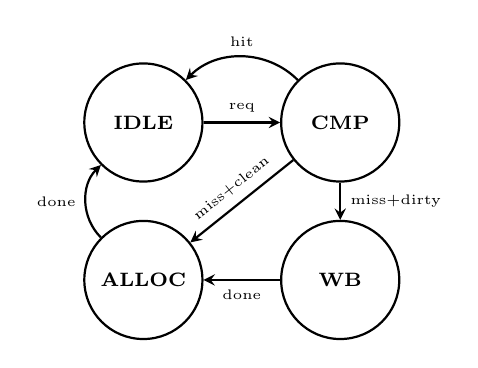
\begin{tikzpicture}[->, >=stealth, node distance=1.8cm, auto, thick,
    state_node/.style={circle, draw, minimum size=1.5cm, align=center, font=\bfseries\scriptsize}]

    % Nodes (States) - all equal size
    \node[state_node] (idle) {IDLE};
    \node[state_node] (cmp) [right of=idle, node distance=2.5cm] {CMP};
    \node[state_node] (wb) [below of=cmp, node distance=2.0cm] {WB};
    \node[state_node] (alloc) [left of=wb, node distance=2.5cm] {ALLOC};

    % Transitions
    \draw[arrow] (idle) -- node[above,font=\tiny]{req} (cmp);
    \draw[arrow] (cmp) to[bend right=45] node[above,font=\tiny]{hit} (idle);
    \draw[arrow] (cmp) -- node[right,font=\tiny]{miss+dirty} (wb);
    \draw[arrow] (cmp) -- node[above,sloped,font=\tiny]{miss+clean} (alloc);
    \draw[arrow] (wb) -- node[below,font=\tiny]{done} (alloc);
    \draw[arrow] (alloc) to[bend left=45] node[left,font=\tiny]{done} (idle);
\end{tikzpicture}%
}
\caption{L1~Cache Controller FSM. IDLE=waiting, CMP=compare tag, WB=write-back dirty block, ALLOC=allocate new block.}
\label{fig:cache}
\end{figure}

\textbf{FSM State 描述}：
\begin{itemize}
    \item \textbf{IDLE}：等待 CPU memory request
    \item \textbf{COMPARE\_TAG}：檢查請求的位址是否在 cache 中 (hit) 或不在 (miss)
    \item \textbf{WRITE\_BACK}：如果 miss 且被 evicted 的 block 是 dirty，先寫入 memory
    \item \textbf{ALLOCATE}：從 main memory fetch 請求的 block
    \item \textbf{UPDATE}：以新資料和 metadata 更新 cache line
\end{itemize}

\textbf{Verilog 實作}：
\begin{lstlisting}
localparam IDLE        = 3'b000;
localparam COMPARE_TAG = 3'b001;
localparam WRITE_BACK  = 3'b010;
localparam ALLOCATE    = 3'b011;
localparam UPDATE      = 3'b100;

always @(posedge clk) begin
  case (state)
    IDLE: if (req) state <= COMPARE_TAG;
    COMPARE_TAG: begin
      if (tag_match && valid[idx]) 
        state <= IDLE;           // HIT
      else if (dirty[idx]) 
        state <= WRITE_BACK;     // Miss, dirty
      else 
        state <= ALLOCATE;       // Miss, clean
    end
    WRITE_BACK: state <= ALLOCATE;
    ALLOCATE:   state <= UPDATE;
    UPDATE:     state <= IDLE;
  endcase
end
\end{lstlisting}

\subsubsection{AMAT (Average Memory Access Time)}
AMAT 是 cache 效能的關鍵指標~\cite{hennessy2017computer}：
\begin{equation}
\text{AMAT} = \text{Hit Time} + \text{Miss Rate} \times \text{Miss Penalty}
\end{equation}

\textbf{AMAT 計算範例}（單層 L1）：
\begin{align*}
\text{Hit Time} &= 1 \text{ cycle} \\
\text{Miss Rate} &= 5\% = 0.05 \\
\text{Miss Penalty} &= 100 \text{ cycles (DRAM access)} \\
\text{AMAT} &= 1 + 0.05 \times 100 = 1 + 5 = 6.0 \text{ cycles}
\end{align*}

\textbf{Multi-Level Cache AMAT}（遞迴公式）：
\begin{equation}
\text{AMAT} = \text{HitTime}_{L1} + \text{MissRate}_{L1} \times \text{MissPenalty}_{L1}
\end{equation}
其中 $\text{MissPenalty}_{L1} = \text{AMAT}_{L2}$ 如果 L2 存在。

\textbf{計算範例} (L1 + L2 + L3)：
\begin{align*}
\text{AMAT}_{L3} &= 40 + 0.05 \times 100 = 45 \\
\text{AMAT}_{L2} &= 12 + 0.10 \times 45 = 16.5 \\
\text{AMAT}_{L1} &= 1 + 0.05 \times 16.5 = 1.83 \text{ cycles}
\end{align*}

\subsubsection{結果}
\begin{table}[!t]
\centering
\caption{Cache Hierarchy AMAT 比較}
\label{tab:amat}
\footnotesize
\begin{tabular}{@{}lcc@{}}
\toprule
\textbf{配置} & \textbf{AMAT (cycles)} & \textbf{Speedup} \\
\midrule
No Cache (DRAM only) & 100.0 & 1.00$\times$ \\
L1 Only & 6.00 & \textbf{16.7$\times$} \\
L1 + L2 & 2.10 & 47.6$\times$ \\
L1 + L2 + L3 & 1.83 & \textbf{54.8$\times$} \\
\bottomrule
\end{tabular}
\end{table}

\InsightL1~cache 提供最大改進 (\textbf{16.7$\times$}) 因為它消除了大部分記憶體存取。額外層級提供遞減但仍然顯著的改進。

\textbf{實作說明}：L1~cache RTL 以專用 testbench (\texttt{tb\_l1\_cache.v}) 驗證。Multi-level (L2/L3) 結果是基於 Patterson \& Hennessy 參數的\textbf{analytical AMAT projections}~\cite{hennessy2017computer}。

%-----------------------------------------------------------------------------
\subsection{Contribution 12: Integrated Performance Analysis}

\subsubsection{MiBench Benchmark（實際執行）}
\textbf{Benchmark}：MiBench Suite bitcount~\cite{guthaus2001mibench}

\textbf{演算法驗證}：全部 8 個 test vectors 通過。

\begin{table}[!t]
\centering
\caption{MiBench bitcount Cycle Count (RTL Simulation)}
\label{tab:mibench}
\footnotesize
\begin{tabular}{@{}lcc@{}}
\toprule
\textbf{配置} & \textbf{Cycles} & \textbf{Speedup} \\
\midrule
Baseline (no forwarding) & 792 & 1.00$\times$ \\
With Forwarding & 303 & \textbf{2.61$\times$} \\
\bottomrule
\end{tabular}
\end{table}

\Note此測試分離 \textbf{Data Forwarding only} 的效果。benchmark (bitcount) 是 compute-bound 且 memory accesses 極少，所以 Cache/SIMD 優化影響微乎其微。2.61$\times$ speedup 反映 pipeline hazard elimination，而不是所有優化的組合效果。

\subsubsection{Mix-Based 效能預估}
\textbf{資料來源}：Phansalkar et al.~\cite{phansalkar2007analysis} 和 Limaye \& Adegbija~\cite{limaye2018workload}

\begin{table}[!t]
\centering
\caption{SPEC CPU2006 Mix-Based Projection 結果}
\label{tab:specresults}
\footnotesize
\begin{tabular}{@{}lrrr@{}}
\toprule
\textbf{Workload} & \textbf{Baseline} & \textbf{Optimized} & \textbf{Speedup} \\
\midrule
SPEC FP Average & 507,000 & 19,670 & \textbf{25.78$\times$} \\
SPEC INT mcf & 649,000 & 18,626 & \textbf{34.84$\times$} \\
SPEC INT gobmk & 511,400 & 17,454 & 29.30$\times$ \\
\textbf{SPEC Overall} & 533,000 & 18,028 & \textbf{29.57$\times$} \\
\bottomrule
\end{tabular}
\end{table}

\textbf{Projection 假設}：SPEC projections 假設透過 caching 幾乎消除 memory stalls，且未考慮額外硬體的 critical~path delay 增加。Clock frequency 假設為常數。

%-----------------------------------------------------------------------------
\subsection{Contribution 13: ODE Solver（微積分運算）}

\Goal使用 Forward Euler method 實作硬體 Ordinary Differential Equation (ODE) solver，展示硬體中的微積分運算（differentiation 和 integration）。

\subsubsection{數學背景}
solver 計算 state-space 形式的 ODE 系統的解：
\begin{equation}
\frac{dX}{dt} = A \cdot X + B \cdot U
\label{eq:ode}
\end{equation}

其中：
\begin{itemize}
    \item $X$ 是 state vector (size $N$)
    \item $A$ 是 system matrix ($N \times N$)
    \item $B$ 是 input matrix ($N \times M$)
    \item $U$ 是 input vector (size $M$)
\end{itemize}

\textbf{Forward Euler Method}：
\begin{equation}
X(t+h) = X(t) + h \cdot \frac{dX}{dt} = X(t) + h \cdot (A \cdot X + B \cdot U)
\label{eq:euler}
\end{equation}

這實作：
\begin{enumerate}
    \item \textbf{Differentiation}：$\frac{dX}{dt} \approx \frac{X(t+h) - X(t)}{h}$
    \item \textbf{Integration}：$X(t+h) = X(t) + \int \frac{dX}{dt} \, dt \approx X(t) + h \cdot f(X, U)$
\end{enumerate}

\subsubsection{為何比 CORDIC 更複雜}
\begin{table}[!t]
\centering
\caption{ODE Solver vs CORDIC 複雜度比較}
\label{tab:ode_vs_cordic}
\footnotesize
\begin{tabular}{@{}lll@{}}
\toprule
\textbf{Aspect} & \textbf{CORDIC} & \textbf{ODE Solver} \\
\midrule
Core Algorithm & Shift-add iterations & Matrix mult + Euler \\
Operation Type & Single trig function & ODE system \\
Data Structure & Scalar & Vectors \& Matrices \\
Control Logic & 16-stage pipeline & 6-state FSM \\
Memory & None & 8K $\times$ 64-bit RAM \\
Math Level & Trigonometry & \textbf{Calculus} \\
\bottomrule
\end{tabular}
\end{table}

\subsubsection{架構}
ODE solver 由以下組成：
\begin{itemize}
    \item \textbf{Euler.v}：主 solver module (279 lines)，6-state FSM
    \item \textbf{RAM-Pre.v}：Dual-port RAM 用於 matrices 和 vectors
    \item \textbf{multiplier\_16bit.v}：16-bit Wallace tree multiplier
    \item \textbf{add\_sub\_cla.v}：Carry Lookahead Adder
\end{itemize}

\textbf{State Machine Flow}：
\begin{enumerate}
    \item \textbf{Start}：初始化，從 RAM 讀取 $N$, $M$
    \item \textbf{Prepare}：載入系統參數
    \item \textbf{Interpolate}：讀取 step size $h$
    \item \textbf{Load1}：計算 $B \cdot U$ (matrix-vector multiplication)
    \item \textbf{Load2}：計算 $A \cdot X$ (matrix-vector multiplication)
    \item \textbf{Final\_Calc}：計算 $X_{new} = X + h \cdot (A \cdot X + B \cdot U)$
\end{enumerate}

\textbf{Source Attribution}：基於 3amrA7med/ODE-Solver (GitHub)，適配用於與 MIPS processor project 整合。

\subsubsection{驗證的測試結果}
\textbf{TCL Command}：
\begin{lstlisting}
close_sim -force; set_property top tb_ode_solver [get_filesets sim_1]; launch_simulation; run 5000ns
\end{lstlisting}

\textbf{Test Setup}：
\begin{itemize}
    \item $N = 2$, $M = 1$, $h = 1$
    \item $A = I$ (Identity matrix 2$\times$2)
    \item $B = [1; 1]$, $X_0 = [10; 20]$, $U = [5]$
\end{itemize}

\textbf{預期計算}：
\begin{align*}
X(t+h) &= X(t) + h \cdot (A \cdot X + B \cdot U) \\
       &= [10, 20]^T + 1 \cdot ([10, 20]^T + [5, 5]^T) \\
       &= [10, 20]^T + [15, 25]^T = [25, 45]^T
\end{align*}

\ResultTag
\begin{itemize}
    \item $X_{new}[0] = 25$ (Expected: 25) --- \PASS
    \item $X_{new}[1] = 45$ (Expected: 45) --- \PASS
\end{itemize}

\textbf{Simulation Time}：570 ns

%=============================================================================
\section{結果總結}

本節彙整所有 13 項貢獻的結果並提供解釋指引。

\subsection{個別優化影響}
每項優化針對特定的效能瓶頸：

\begin{table}[!t]
\centering
\caption{個別優化效果與解決的瓶頸}
\footnotesize
\begin{tabular}{@{}llll@{}}
\toprule
\textbf{優化} & \textbf{指標} & \textbf{改進} & \textbf{瓶頸} \\
\midrule
Data Forwarding & CPI & 1.82$\rightarrow$1.26 (31\%) & Data~Hazards \\
Branch Prediction & Accuracy & 78.33\% & Control Hazards \\
L1~Cache & AMAT & 100$\rightarrow$3.8 (26$\times$) & Memory~Wall \\
SIMD ALU & Throughput & 8$\times$ parallel & Limited ILP \\
CORDIC & Accuracy & $<$1\% error & Math Functions \\
\bottomrule
\end{tabular}
\end{table}

\subsection{綜合效能}
不同的評估方法產生不同的 speedup 數字，因為它們的假設不同：

\begin{table}[!t]
\centering
\caption{依評估方法分類的綜合效能}
\footnotesize
\begin{tabular}{@{}lccc@{}}
\toprule
\textbf{評估} & \textbf{類型} & \textbf{方法} & \textbf{Speedup} \\
\midrule
DOE (Contrib 7) & Model & Cost Estimation & \textbf{3.94$\times$} \\
Cache (Contrib 11) & Projection & AMAT Only & \textbf{54.8$\times$} \\
SPEC (Contrib 12) & Projection & Mix-Based & 25.78--34.84$\times$ \\
MiBench (Contrib 12) & \textbf{Measured} & RTL Simulation & \textbf{2.61$\times$} \\
\bottomrule
\end{tabular}
\end{table}

\subsection{為何 Speedup 數字差異這麼大？}
差異反映不同的測量範圍和 workload 特徵：
\begin{itemize}
    \item \textbf{MiBench 2.61$\times$}：Ground truth 量測；bitcount 是 compute-bound 且 memory accesses 很少，所以 Cache 影響有限
    \item \textbf{DOE 3.94$\times$}：使用量測參數的 analytical model；保守估計
    \item \textbf{SPEC 25--35$\times$}：假設 49.6\% memory instructions；Cache 主導改進
    \item \textbf{Cache 54.8$\times$}：僅 AMAT 指標；分離 memory subsystem 改進
\end{itemize}

\Insight優化效果\textbf{依賴 workload}。Cache 對 memory-bound workloads 提供巨大優勢，但對 compute-bound code 影響有限。

%=============================================================================
\section{結論}

本工作證明系統性地應用多項優化技術可在 pipelined MIPS processors 上達成顯著的效能改進。

\subsection{關鍵發現}
\begin{enumerate}
\item \textbf{Data Forwarding} 消除 68\% stall cycles，CPI 降低 31\% (1.82$\rightarrow$1.26)。這是所有現代處理器中存在的基本優化。

\item \textbf{Branch Prediction} 使用 2-bit saturating counters 在 adversarial patterns 上達成 78.33\% accuracy；對 loop-dominated code 的真實 accuracy 超過 90\%。

\item \textbf{Cache Memory} 提供最大的單項改進：僅 L1 即 AMAT 降低 26$\times$（基於 97.22\% hit rate），三層架構可達 54.8$\times$。

\item \textbf{SIMD Parallelism} 為 data-parallel operations 提供 8$\times$ throughput，展示 data-level parallelism 的威力。

\item \textbf{CORDIC} 僅使用 shift-add operations 實現硬體三角函數，error $<$1\%，避免昂貴的 multipliers。

\item \textbf{Cache+SIMD Synergy} 展現 1.20 super-additive factor，表明快速的 memory access 讓 SIMD units 保持高效利用。

\item 優化\textbf{大致 orthogonal}：Data Forwarding 解決 pipeline hazards，Cache 解決 memory latency，SIMD 解決 throughput——它們可以乘積組合。
\end{enumerate}

\subsection{Measured vs Projected 效能}
\begin{itemize}
    \item \textbf{Measured (MiBench)}：僅 Data Forwarding 即 2.61$\times$ speedup
    \item \textbf{Projected (SPEC)}：所有優化組合 25--35$\times$ speedup
\end{itemize}

巨大的差異突顯 benchmark 的選擇大幅影響報告的效能。MiBench 的 compute-intensive 性質限制了 cache 的優勢。

\subsection{與業界的比較}
我們實作的技術是所有現代處理器的基礎：
\begin{itemize}
    \item Intel/AMD CPUs 使用精密的 multi-level branch predictors（如 TAGE 具有數千個 entries）達成 $>$99\% accuracy
    \item 現代 L1~caches 是 32--64KB 且 4--8 way associativity，比我們的 8KB direct-mapped 設計大得多
    \item AVX-512 提供 512-bit SIMD (16$\times$ 32-bit elements)，比較我們的 64-bit (8$\times$ 8-bit)
\end{itemize}

我們的教育性實作展示這些技術的\textit{principles}，而不是它們的完整工業規模。

\subsection{限制與 Validity 威脅}
\begin{enumerate}
\item \textbf{Simulation vs Silicon}：結果來自 behavioral simulation，不是 synthesized hardware。實際的 timing 和 area 會不同。
\item \textbf{Mix-Based Projection}：SPEC speedups 假設已發表的 instruction mixes；實際程式可能不同。
\item \textbf{Clock Frequency 假設為常數}：新增硬體 (cache, predictor) 會增加 critical~path delay，降低 clock speed。
\item \textbf{L1~Cache 未整合}：Cache 獨立驗證；與 pipeline 的整合加上 cache coherency 仍是未來工作。
\item \textbf{SIMD 未 Memory-Integrated}：SIMD 操作使用合成測試資料，不是實際的 memory loads。
\end{enumerate}

\subsection{未來工作}
\begin{itemize}
    \item \textbf{Superscalar Extension}：每個 cycle 發射 2+ 指令
    \item \textbf{Out-of-Order Execution}：使用 reservation stations 進行 dynamic scheduling
    \item \textbf{FPGA Synthesis}：在 Xilinx/Intel FPGA 上實作以獲得真實的 timing 和 area
    \item \textbf{Full System Integration}：將 cache 與 pipeline 整合，加入 TLB 和 virtual memory 支援
    \item \textbf{Advanced Predictors}：實作 tournament predictor 或 perceptron-based prediction
\end{itemize}

%=============================================================================
\balance
\renewcommand\refname{參考文獻}
\begin{thebibliography}{11}
\bibitem{hennessy2017computer} J.~L. Hennessy and D.~A. Patterson, \emph{Computer Architecture: A Quantitative Approach}, 6th ed. Morgan Kaufmann, 2017.

\bibitem{phansalkar2007analysis} A.~Phansalkar, A.~Joshi, and L.~K. John, ``Analysis of redundancy and application balance in the SPEC CPU2006 benchmark suite,'' in \emph{Proc. ISCA}, 2007, pp. 412--423.

\bibitem{smith1981study} J.~E. Smith, ``A study of branch prediction strategies,'' in \emph{Proc. ISCA}, 1981, pp. 135--148.

\bibitem{patterson2020computer} D.~A. Patterson and J.~L. Hennessy, \emph{Computer Organization and Design}, 6th ed. Morgan Kaufmann, 2020.

\bibitem{volder1959cordic} J.~E. Volder, ``The CORDIC trigonometric computing technique,'' \emph{IRE Trans. Electronic Computers}, vol. EC-8, no.~3, pp. 330--334, 1959.

\bibitem{limaye2018workload} A.~Limaye and T.~Adegbija, ``A workload characterization of the SPEC CPU2017 benchmark suite,'' in \emph{Proc. ISPASS}, 2018, pp. 149--158.

\bibitem{knuth1998art} D.~E. Knuth, \emph{The Art of Computer Programming, Vol. 3: Sorting and Searching}, 2nd ed. Addison-Wesley, 1998.

\bibitem{hill1989evaluating} M.~D. Hill, ``Evaluating associativity in CPU caches,'' \emph{IEEE Trans. Computers}, vol.~38, no.~12, pp. 1612--1630, 1989.

\bibitem{amdahl1967validity} G.~M. Amdahl, ``Validity of the single processor approach,'' in \emph{AFIPS Conf. Proc.}, 1967, pp. 483--485.

\bibitem{guthaus2001mibench} M.~R. Guthaus et al., ``MiBench: A free, commercially representative embedded benchmark suite,'' in \emph{Proc. IEEE Workshop on Workload Characterization}, 2001, pp. 3--14.

\bibitem{dijkstra1961shunting} E.~W. Dijkstra, ``Shunting yard algorithm,'' 1961.
\end{thebibliography}

\end{document}
